\documentclass[a4paper,12pt]{report}
\usepackage{styles/fbe_tez}
\usepackage[utf8]{inputenc}
\usepackage[T1]{fontenc}
\usepackage{lmodern}
\usepackage{amsmath, amssymb}
\usepackage[bottom]{footmisc}
\usepackage{cite}
\usepackage{url}
\usepackage{booktabs}
\usepackage{tabularx}
\usepackage{ragged2e}
\usepackage{enumitem}
\usepackage{microtype}
\usepackage{tikz}
\usetikzlibrary{shapes,arrows.meta,positioning}
\usepackage[hidelinks]{hyperref}

\renewcommand{\labelenumi}{(\roman{enumi})}
\setlist{itemsep=2pt,topsep=3pt}
\emergencystretch=3em

\begin{document}

\title{CMPE 492 \\ A THREE-LAYER EVALUATION OF SPEECH-TO-TEXT, LLM-BASED TERMINOLOGY EXTRACTION, AND GENERATIVE VIDEO-ANIMATION FOR MULTILINGUAL EDUCATION}
\author{
Ali Ayhan G{\"{u}}nder \\ \\
Advisor: \\
Prof. Fatih Alag{\"{o}}z
}
\date{November 2026}
\maketitle

\pagenumbering{roman}
\tableofcontents
\newpage

% =========================================================================
\chapter{INTRODUCTION}
\pagenumbering{arabic}

Individualized instruction tailored to a learner's prerequisite readiness outperforms conventional classroom teaching by two standard deviations \cite{bloom1984}, yet human one-to-one tutoring does not scale to Massive Open Online Courses (MOOCs). In university lectures, instructors continuously introduce domain-dense terminology without pausing to scaffold foundational prerequisites, inducing cognitive overload for beginner and multilingual learners \cite{conde2016,xu2024}.

This project designs and empirically evaluates a three-layer artificial intelligence pipeline for Turkish and English educational scaffolding: (i) multilingual Automatic Speech Recognition (ASR), (ii) LLM-based terminology extraction, prerequisite dependency mapping, and CEFR-B1 simplification, and (iii) Socratic multi-turn tutoring with on-demand generative explainer animations.

\section{Broad Impact}
By transforming unstructured lecture audio into prerequisite-aware, CEFR-calibrated Turkish and English study aids, the system lowers linguistic and conceptual barriers for first-generation and non-native engineering students. Running quantized 2B--14B models locally and on institutional HPC hardware also supports data sovereignty and low-cost university deployment.

\section{Ethical Considerations}
Educational AI assistants must avoid hallucinated definitions, unauthorized leakage of student transcripts, and direct exam-answer generation. All experiments use anonymized or synthetic learner personas, enforce strict Turkish script guardrails, and evaluate anti-cheating Socratic deflection rather than direct homework completion.

% =========================================================================
\chapter{PROJECT DEFINITION AND PLANNING}

\section{Project Definition}
The project delivers an end-to-end lecture scaffolding prototype covering speech transcription, concept graph extraction, CEFR-B1 readability adaptation, and preference-aligned Socratic tutoring, validated primarily on Turkish Occupational Health and Safety (\.{I}SG) and multi-domain university benchmarks.

\section{Project Planning}

\subsection{Project Time and Resource Estimation}
Development and experimentation are organized into three phases on the Bo\u{g}azi\c{c}i University HPC cluster (\texttt{ultramarine}, NVIDIA A40 48\,GB):
\begin{itemize}
    \item \textbf{Phase 1 --- Acoustic \& Extraction Baselines (Completed):} ASR benchmarking, multilingual terminology extraction, and 7-tier scaling law profiling ($0.5\text{B} \to 72\text{B}$).
    \item \textbf{Phase 2 --- Pedagogical Alignment \& Guardrails (Completed):} QLoRA fine-tuning, SFT overfitting diagnosis, on-policy DPO training, and Non-Latin logit masking.
    \item \textbf{Phase 3 --- Final Validation \& Thesis Delivery (Planned / In Progress):} Higher-capacity 14B judge auditing, out-of-domain (OOD) transfer testing, anti-cheating DPO guardrails, and final report defense.
\end{itemize}

\subsection{Success Criteria}
Key quantitative targets include low-WER multilingual transcription ($\text{WER} < 0.10$), high terminology extraction F1 ($\ge 0.85$), reliable CEFR readability adherence, $\ge 80\%$ misconception resolution in multi-turn Socratic tutoring, and $0.00\%$ non-Latin script leakage.

\subsection{Risk Analysis}
\begin{itemize}
    \item \textbf{SFT Template Overfitting \& Alignment Tax:} Naive multi-turn SFT can memorize rigid templates and degrade JSON/CEFR calibration. \textit{Mitigation:} Task-separated prompting and on-policy DPO.
    \item \textbf{Multilingual Script Drift:} Multilingual LLMs occasionally emit CJK or Cyrillic tokens under noisy Turkish student inputs. \textit{Mitigation:} Vocabulary-level \texttt{NonLatinBlockLogitsProcessor}.
    \item \textbf{Adversarial Cheat Pressure:} Instruction-following tutors may leak direct exam answers. \textit{Mitigation:} Planned anti-cheating preference pairs (\texttt{dpo\_v3\_guardrail}).
\end{itemize}

% =========================================================================
\chapter{RELATED WORK}

Modern multilingual ASR architectures such as Whisper \cite{radford2023,whisper-turbo} and Qwen3-ASR \cite{qwen3asr2026} enable accurate transcription of technical lectures. In Automatic Terminology Extraction (ATE), statistical multi-word metrics \cite{frantzi2000} have largely been superseded by instruction-tuned LLMs capable of structured extraction and readability adaptation. Meanwhile, intelligent tutoring systems grounded in Knowledge Tracing \cite{corbett1995} and adaptive hypermedia \cite{brusilovsky2007} demonstrate that step-based Socratic scaffolding yields significantly higher learning gains than direct answer delivery \cite{vanlehn2011}. Our work bridges these three threads into a unified, preference-aligned Turkish educational pipeline.

% =========================================================================
\chapter{METHODOLOGY}

Figure~\ref{fig:midterm_pipeline} summarizes the three-layer architecture evaluated in this project:
\begin{enumerate}
    \item \textbf{Layer 1 (Acoustic):} Evaluates \texttt{Whisper-large-v3-turbo} and \texttt{Qwen3-ASR 1.7B} on technical lecture audio.
    \item \textbf{Layer 2 (Semantic):} Extracts canonical domain terms, constructs prerequisite Directed Acyclic Graphs (DAGs), and generates CEFR-B1 Turkish explanations.
    \item \textbf{Layer 3 (Pedagogical Alignment):} Replaces brittle SFT templates with on-policy Direct Preference Optimization (DPO) and a \texttt{NonLatinBlockLogitsProcessor} ($51{,}167$ blocked non-Latin tokens) for fluent Turkish Socratic dialogue.
\end{enumerate}

\begin{figure}[htbp]
\centering
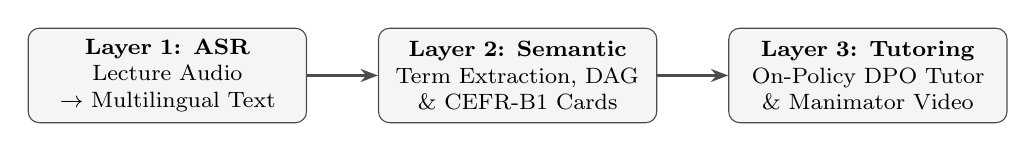
\begin{tikzpicture}[
    node distance=0.8cm and 0.9cm,
    box/.style={rectangle, rounded corners=4pt, draw=black!70, fill=gray!8, text width=3.3cm, align=center, font=\footnotesize, minimum height=1.2cm},
    arr/.style={-{Stealth[length=2.2mm]}, thick, black!70}
]
\node[box] (asr) {\textbf{Layer 1: ASR}\\Lecture Audio\\$\to$ Multilingual Text};
\node[box, right=of asr] (sem) {\textbf{Layer 2: Semantic}\\Term Extraction, DAG\\\& CEFR-B1 Cards};
\node[box, right=of sem] (tut) {\textbf{Layer 3: Tutoring}\\On-Policy DPO Tutor\\\& Manimator Video};
\draw[arr] (asr) -- (sem);
\draw[arr] (sem) -- (tut);
\end{tikzpicture}
\caption{Three-layer pipeline of the EduTerm multilingual educational scaffolding system.}
\label{fig:midterm_pipeline}
\end{figure}

% =========================================================================
\chapter{REQUIREMENTS SPECIFICATION}

Core functional requirements cover: (FR1) multilingual lecture audio transcription, (FR2) structured JSON terminology and prerequisite DAG extraction, (FR3) CEFR-B1 readability adaptation, and (FR4) multi-turn Socratic misconception resolution. Non-functional requirements specify deterministic Turkish-only script output ($0\%$ non-Latin leakage), low-VRAM 4-bit NF4 compatibility on single-GPU nodes, and strict schema validity for downstream UI rendering.

% =========================================================================
\chapter{DESIGN}

The system decouples heavy semantic extraction from interactive tutoring. Lecture transcripts are processed once by Layer~2 to populate a prerequisite DAG and CEFR-B1 concept cards. During live tutoring (Layer~3), the tutor receives only the target concept, prerequisite context, and student turn, while decoding passes through \texttt{NonLatinBlockLogitsProcessor} to prevent CJK or Cyrillic drift without modifying base model weights.

% =========================================================================
\chapter{IMPLEMENTATION AND TESTING}

All training and evaluation runs up to the midterm milestone were executed on the Bo\u{g}azi\c{c}i HPC cluster (\texttt{ultramarine}, NVIDIA A40 48\,GB) using PyTorch, Hugging Face \texttt{transformers}, \texttt{bitsandbytes} 4-bit NF4 quantization, and PEFT QLoRA adapters. Multi-turn tutoring was tested with \texttt{Kumru-2B} and unquantized \texttt{Qwen2.5-7B-Instruct} (\texttt{bfloat16}) student simulators across $3$ random seeds and $3$ learner personas, paired with an alignment tax audit across $36$ CEFR (B1/B2/C1) and $12$ JSON schema probes.

% =========================================================================
\chapter{RESULTS}

Tables~\ref{tab:midterm_summary} and~\ref{tab:midterm_alignment} summarize our verified midterm milestones and alignment comparison.

\begin{table}[htbp]
\centering
\small
\caption{Verified Midterm Experimental Milestones Across Pipeline Layers.}
\label{tab:midterm_summary}
\scriptsize\setlength{\tabcolsep}{4pt}
\begin{tabularx}{\textwidth}{>{\RaggedRight\arraybackslash}l >{\RaggedRight\arraybackslash}X >{\RaggedRight\arraybackslash}X}
\toprule
\textbf{Pipeline Component} & \textbf{Evaluated Configuration} & \textbf{Primary Verified Outcome} \\
\midrule
Layer 1: ASR & \texttt{Qwen3-ASR 1.7B} on lecture audio & $\text{WER} = 0.061$, $\text{CER} = 0.015$ \\
Layer 2: Terminology & \texttt{Qwen2.5-7B} extraction benchmark & Term extraction $\text{F1} = 0.887$ \\
Scaling \& QLoRA & 7-tier ($0.5\text{B} \to 72\text{B}$) + \texttt{EduTerm-14B} & $62.5\%$ Bloom accuracy; $91.7\%$ CEFR adherence \\
Live Socratic Tutoring & \texttt{onpolicy\_dpo\_v2} (3-seed \texttt{7B-bf16}, $n=216$) & \textbf{86.11\%} misconception resolution ($0.00\%$ leakage) \\
\bottomrule
\end{tabularx}
\end{table}

To isolate the impact of preference alignment on both tutoring resolution and core model capabilities (CEFR readability calibration and structured JSON generation), Table~\ref{tab:midterm_alignment} contrasts our base, SFT, task-separated hybrid, and on-policy DPO configurations.

\begin{table}[htbp]
\centering
\small
\caption{Pedagogical Alignment and Alignment Tax Comparison.}
\label{tab:midterm_alignment}
\scriptsize\setlength{\tabcolsep}{3.5pt}
\begin{tabularx}{\textwidth}{>{\RaggedRight\arraybackslash}Xcccc}
\toprule
\textbf{Condition / Adapter} & \textbf{Resolved Rate} & \textbf{Non-Latin Leakage} & \textbf{CEFR Comp.} & \textbf{JSON Valid} \\
\midrule
\texttt{base\_14b} (No Alignment) & 75.00\%--77.78\% & --- & \textbf{69.44\%} & \textbf{100.0\%} \\
SFT (\texttt{cefr} / \texttt{socratic\_v2}) & 41.67\% (Kumru) & $>0\%$ (CJK) & 36.11\%--44.44\% & 50.0\%--100.0\% \\
\texttt{task\_separated\_hybrid} & 82.41\% (\texttt{7B-bf16}) & \textbf{0.00\%} & 69.44\% (Base) & \textbf{100.0\%} \\
\textbf{\texttt{onpolicy\_dpo\_v2}} & \textbf{86.11\%} (\texttt{7B-bf16}) & \textbf{0.00\%} & 61.11\% & \textbf{100.0\%} \\
\bottomrule
\end{tabularx}
\end{table}

Key takeaways: (1) \texttt{onpolicy\_dpo\_v2} achieved \textbf{86.11\%} misconception resolution across $216$ paired 3-seed \texttt{7B-bf16} sessions with \textbf{0.00\%} non-Latin leakage; (2) unlike SFT adapters (which dropped JSON validity to $50.0\%$ and CEFR compliance to $36.11\%$), DPO preserved \textbf{100.0\%} JSON schema validity and strong B1--C1 readability contrast.

% =========================================================================
\chapter{CONCLUSION}

By the midterm milestone, the core three-layer pipeline, QLoRA scaling benchmarks, Non-Latin logit guardrail, and on-policy DPO tutoring alignment have been implemented and empirically validated. For the final phase (planned), we will complete a 14B high-capacity judge audit, out-of-domain (OOD) transfer evaluations across CS, KVKK, Banking, and Electrical Engineering concepts, and anti-cheating guardrail DPO (\texttt{dpo\_v3\_guardrail}) prior to final thesis defense.

\bibliographystyle{styles/fbe_tez_v11}
\bibliography{references}

\end{document}
